\documentclass{llncs}
\usepackage{makeidx}
\usepackage[spanish]{babel}
\usepackage[utf8]{inputenc}
\usepackage{amsmath}
\usepackage{url}
\usepackage{fancyvrb}
\usepackage[spanish]{babelbib}
\usepackage{graphicx}

\graphicspath{ {img/} }

\urldef{\mails}\path|{fbarrios,fjlopez}@fi.uba.ar| 

\newtheorem{definicion}{Definición} 

\begin{document}

\frontmatter

\title{TextRank Variations for Automated Summarization}
\titlerunning{Variantes de TextRank} 


\maketitle

\begin{abstract}
This article describes the proposal and analysis of new variants of the TextRank algorithm for automated summarization of texts. We describe the generalities of the TextRank algorithm on its original version and the different variations that we tested. Some of these variants achieve a significative improvement over the original algorithm using the same metrics as dataset as the original publication. 
\keywords{TextRank, resumen, automático}

\end{abstract}

\section{Introducción}
We can describe the process of automated summarization as the extraction of the most important sentences in a document. Using different levels of compression a summarized version of the document of arbitrary length can be obtained. The TexRank algorithm is one of the most used methods for this task. TextRank builds a graph of sentendes for a document and then applies PageRank to obtain a score for each sentence. The sentences with higher score are then used for the summary presented in the order in which they appear in the text. Using different schemes for the construction of the graph we can achieve different results. In this article we describe several different proposals for the construction of the TextRank graph and report the results obtained with them.
The first section of this article describes previous work in the area and the TextRank algorithm in general. Then we describe the different metrics used for the evaluation of the results obtained from the proposed changes and the datasets used for these tests. Finally we report the results obtained for the different variations of the algorithm.
\section{Trabajo previo}
The field of automated summarization has advanced in a significative way since the late 60's 
\cite{miranda}. Traditional methods for text summarization analyze the frequency of words or sentences in the first paragraphs of the text to identify the most important ones. Several statistical models have been developed based on training corpuses to combine different heuristics using keywords, position and length of sentences, word frequency and titles \cite{hovy}. Other mmethods are based in the representation of the text as a graph: the most important sentences are the most connected ones in the graph and are used for the summaryzation \cite{barzilay}. On a different approach some algorithms analyze the semantic strcutre of the different textual units in a document with the goal of sepparating those that take a significative role in the representation of the document \cite{marcu}.

The algorithms based on the construction of a graph to represent text used different information retrieval techniques to identify similar sentences and determine the most important ones to build a final summary \cite{salton}. The algorithm developed by Mihalcea and Tarau \cite{mihalcea-tarau} and also Erkan and Radev \cite{erkan} is based in ranking the lexical units of the text (sentences or words). This method is the one adopted by TextRank.

\section{TextRank}

\subsection{Description}
TextRank is an unsupervised algorithm based in graphs for the automated summarization of texts that can also be used to obtain the most important keywords in a document. It was introduced in 2004 by Rada Mihalcea and Paul Tarau on its paper “TextRank: Bringing Order into Texts”  \cite{mihalcea-tarau}

The algorithm applies a variation of PageRank \cite{pageetal98} over a graph constructed specifically for the task of summarization. This method allows to understand the structure of the document identifying its principal concepts without the need of previous training. Since the algorithm is based on PageRank it uses the idea of relevance/ranking of the elements in the graph, the most important elements are the ones that better describe the text. This approach allows TextRank to build summaries without the need of a training corpus or labeling and allows the use of the algorithm in different languages as long as there is a way to build the graph of sentences for it.

\subsection{Text as a Graph}
TextRank models any document as a graph, it can use words or sentences as the different nodes in the graph. Sentences are used for automated summarization and words for keyword extraction. After extracting sentences as noces in a graph the algorithm needs to build edges between its nodes. A function to compute the simmilarity of sentences is then needed. The simmilarity function is used to weight the graph edges, the higher the simmilarity between sentences the more important the edge between them will be in the graph. In the domain of a Random Walker as used frequently in PageRank we can say that we are more likely to go from one sentence to another if those sentences are very similar. 

The simmilarity function can use several different ideas, it can be based in the semantic of the sentences, in their proximity in the text, common words, and many other different metrics. The idea of this article is to experiment with different simmilarity functions and report the results obtained when used along with TextRank.

The steps needed to build a summary using TextRank are:

\begin{enumerate}
\item Identificar las unidades del texto (palabras u oraciones) y agregarlas al grafo como vértices.
\item Identificar relaciones que conectan a estas unidades, y agregarlas al grafo como aristas entre los vértices. Las aristas pueden ser dirigidas o no, y ponderadas o no.
\item Aplicar PageRank para asignarle un puntaje a cada vértice.
\item Ordenar los vértices de acuerdo al puntaje y utilizarlo para armar el resumen de acuerdo a algún criterio.
\end{enumerate}

\subsection{Generación de resúmenes automáticos}
El problema de la extracción de oraciones apunta a identificar las secuencias más representativas del texto. Para este caso, las unidades tomadas para aplicar el algoritmo serán oraciones completas \cite{introductionir}.

Inicialmente, se construye un grafo en base al texto. Cada oración se considera como un vértice, y para asignarles peso a las aristas se debe definir una función de semejanza entre dos oraciones dadas. Esta función será la que dicte cuánto una oración “recomienda” a otra, dependiendo de la similitud entre sus contenidos por abordar los mismos conceptos.
    
La función utilizada se define formalmente de la siguiente manera:


\begin{definicion}
Sean $S_i$, $S_j$ dos oraciones representadas por un conjunto de $n$ palabras que en 
$S_i$ aparecen como $S_i = w_{1}^{i}, w_{2}^{i},..., w_{n}^{i}$. La función de similitud para $S_i$, $S_j$ se define como:


\begin{equation}
Similitud(S_{i},S_{j}) = \frac{ | \{   w_{k} | w_{k} \in S_{i} \& w_{k} \in S_{j}   \}  | }    
                              {  log(|S_{i}|) + log(|S_{j}|)  }
\end{equation}


\end{definicion}
    
El resultado de este proceso es el texto representado como un grafo ponderado y altamente denso. A partir de este grafo se aplica PageRank para calcular la relevancia de cada vértice, es decir de cada oración del texo.

Luego de aplicar el algoritmo de relevancia/priorización se seleccionan las oraciones con mayor puntaje para incluirlas en el resumen. Estas, finalmente, se presentan de acuerdo al orden de aparición en el texto original.


\section{Experimentos}

\subsection{Evaluación}
Se decidió usar la base de datos de la tarea de generación de resúmenes automáticos de la conferencia DUC (Document Understanding Conference) del año 2002 \cite{duc2002-guidelines}, este el mismo corpus que el usado en la presentación del algoritmo TextRank en \cite{mihalcea-tarau}. El corpus cuenta con 567 documentos que fueron resumidos a cerca del 20\% de su tamaño.

Para llevar a cabo la evaluación se usó la versión 1.5.5 del paquete de métricas ROUGE \cite{Lin2004a}. Se utilizó la configuración usada en DUC, calculando sólo las mediciones ROUGE-1, ROUGE-2 y ROUGE-SU4 en un intervalo de confianza del 95\% y aplicando un método de \textit{stemming}. Se obtuvo un único puntaje promediando los tres valores.

Para verificar el funcionamiento de todo el conjunto se desarrolló el método de referencia (\textit{baseline}) usado en \cite{mihalcea-tarau}, que construye el resumen extrayendo las primeras oraciones de cada artículo. Se comprobó que los resultados fueron similares: la versión original de TextRank mejora al \textit{baseline} en un 2,3\% aproximadamente.

\subsection{Propuestas}
En la siguiente sección se describen las variantes que se probaron sobre el algoritmo original de
TextRank. Principalmente estas modificaciones apuntan a cambiar la forma en la cual se calculan las distancias entre las oraciones de los textos. Diferentes métricas arrojaron diferentes resultados y algunas de éstas variantes lograron una mejora significativa sobre el algoritmo original.

\subsubsection{Subcadena común}
Dadas dos frases, el problema de la subcadena común más larga consiste en identificar la secuencia de caracteres de mayor extensión presente en ambas. Por ejemplo, entre “la cocina verde” y “una cocina vale más si es verde”, la secuencia más larga es “a cocina v”.

La propuesta consiste en modificar la función de distancia de la implementación original y reemplazarla por el largo de la subcadena común más larga. En el ejemplo anterior, la similitud sería de 10, dado que es el largo de la secuencia “a cocina v”.

Cabe destacar el parecido de esta métrica con los métodos de evaluación ROUGE.


\subsubsection{Similitud coseno}
La similitud coseno es una medida de la similitud existente entre dos vectores en un espacio que posee un producto interior con el que se evalúa el valor del coseno del ángulo comprendido entre ellos. Para poder hacer uso de esta “distancia” se utiliza el modelo vectorial es decir que se modelan a los documentos como vectores.

Este modelo algebraico es utilizado para representar documentos en lenguaje natural de una manera formal mediante el uso de vectores en un espacio multidimensional. La teórica básica es que el parecido de un documento frente a otro puede calcularse usando la similitud coseno. 

Este modelo está basado en favorecer la dirección a la cuál apuntan los documentos independientemente de su longitud. Textos que hablan de los mismos temas pero tienen diferente longitud pueden tener una distancia angular muy pequeña resultando en un coseno cercano a uno que es el valor máximo cuando el ángulo entre los documentos es cero.

La propuesta se basa en aplicar este modelo para tratar a cada oración del texto como un vector n-dimensional (siendo n la cantidad de palabras distintas presentes en el documento), y luego compararlas utilizando la similitud coseno. Las entradas de cada vector estarán compuestas por el resultado de aplicar la función “frecuencia de término -- frecuencia inversa de documento” (TF--IDF de sus siglas en inglés) a cada palabra de la oración representada.

Tomando como ejemplo el documento “Esta bien. Todo bien.”, las oraciones quedarían modeladas como vectores de la siguiente forma:

\begin{Verbatim}[xleftmargin=3em]
v1=[ TFIDF("Esta") , TFIDF("bien") ,       0       ]
v2=[       0       , TFIDF("bien") , TFIDF("Todo") ]
\end{Verbatim}

Dado que la imagen de la función TFIDF está contenida en el intervalo [0,1], todos los vectores quedan conformados por entradas no negativas, haciendo que ninguna similitud sea menor a cero. 

\subsubsection{BM25}
Okapi BM25 es una función de ranking utilizada para la asignación de relevancia a los documentos en un buscador. 
Está basada en los modelos probabilísticos de Recuperación de información, y actualmente 
representa el estado del arte en algoritmos de recuperación de documentos basados en frecuencia de término -- frecuencia inversa de documento.

\begin{definicion}
Dadas dos oraciones R, S, BM25 se define como:

\begin{equation}
BM25(R,S) = \sum_{i=1}^{n} IDF(s_i) \cdot \frac{f(s_i, R) \cdot (k_1 + 1)}{f(s_i, R) + k_1 \cdot (1 - b + b \cdot \frac{|R|}{avgDL})}
\end{equation}

donde $k$ y $b$ son parámetros que valen $k = 1,2$ y $b = 0,75$, y $avgDL$ es el largo promedio de las oraciones en el texto.
\end{definicion}

Esta función contempla la frecuencia inversa del documento de manera tal que si una palabra aparece en más de la mitad de los textos, el valor para ese término se vuelve negativo. Dado que este comportamiento no es deseable para esta aplicación, se utiliza la siguiente fórmula:
                
\begin{equation}
 IDF(q_i) =
  \begin{cases}
       log(N - n(q_i) + 0.5) - log(n(q_i) + 0.5)    & \text{si }  n(q_i) > N/2\\
       \varepsilon \cdot avgIDF                     & \text{si }  n(q_i) \leq N/2\\
  \end{cases}
\end{equation}                
                
donde $\varepsilon$ ronda entre 0,5 y 0,30 y $avgIDF$ es el idf promedio para todos los términos.
También se ensayaron alternativas como igualar a cero el resultado en caso de ser negativo, o reemplazar la función inversa por una similar, cuyo resultado es no negativo, o estrictamente positivo. 

Existe una variante a BM25 llamada BM25+. Esta repara deficiencias relacionadas a la frecuencia de término y a la penalización a documentos largos frente a documentos cortos irrelevantes.

La propuesta consistió en aplicar BM25 y BM25+ entre las oraciones de un texto, a fin de ordenarlas de acuerdo a su relevancia.


\subsection{Resultados Obtenidos}
Los mejores resultados se obtuvieron usando BM25 y BM25+. El incremento más alto se logró al reemplazar los valores negativos por la constante $\varepsilon$ = 0.25, dando una mejora total de 2,92\% para BM25 y 2,60\% para BM25+. Inicialmente se obtuvieron valores cercanos al 1,30\%, pero dado que esta función contempla el uso de \textit{stopwords} se procedió a eliminar la etapa de filtrado del preprocesamiento del texto, alcanzado así resultados sobresalientes. En el Cuadro 1 se detallan las alternativas ensayadas.

\begin{table}
\caption{Resultados de las distintas propuestas}
\begin{center}
\begin{tabular}{l*{5}{c}r}
\hline
\rule{0pt}{12pt}
Método & ROUGE-1 & ROUGE-2 & ROUGE-SU4 & Mejora \\[2pt]
\hline\rule{0pt}{12pt}\mbox{}\par\nobreak
BM25 (Neg a epsilon) & 0.4042 & 0.1831 & 0.2018 & 2,92\% \\
BM25+ (Neg a epsilon) & 0.404 & 0.1818 & 0.2008 & 2,60\% \\
Cosine TF-IDF & 0.4108 & 0.177 & 0.1984 & 2,54\% \\
BM25+ (IDF = log(N/NI)) & 0.4022 & 0.1805 & 0.1997 & 2,05\% \\ 
BM25 (IDF = log(N/NI)) & 0.4012 & 0.1808 & 0.1998 & 1,97\% \\ 
Longest Common Substring & 0.402 & 0.1783 & 0.1971 & 1,40\% \\
BM25+ (Neg a cero) & 0.3992 & 0.1803 & 0.1976 & 1,36\% \\ 
BM25 (Neg a cero) & 0.3991 & 0.1778 & 0.1966 & 0,89\% \\
\textbf{TextRank} & \textbf{0.3983} & \textbf{0.1762} & \textbf{0.1948} & \textbf{--}\\
BM25 & 0.3916 & 0.1725 & 0.1906 & -1,57\% \\
BM25+ & 0.3903 & 0.1711 & 0.1894 & -2,07\% \\
DUC Baseline & 0.39 & 0.1689 & 0.186 & -2,84\% \\ [2pt]
\hline
\end{tabular}
\end{center}
\end{table}

Los tiempos de ejecución también se superaron. Se pudieron procesar los 567 documentos de la base de datos de DUC2002 utilizando 84\% del tiempo requerido por la versión original.

El resultado de la métrica de similitud coseno también fue satisfactoria, presentando una mejora de 2,54\% por sobre el método original. A su vez, los métodos de secuencias de máxima longitud también mostraron una mejora considerable: cerca del 1,40\% por sobre TextRank. En la Figura 1 se comparan los distintas técnicas.

\begin{figure}[h!]
    \centering
    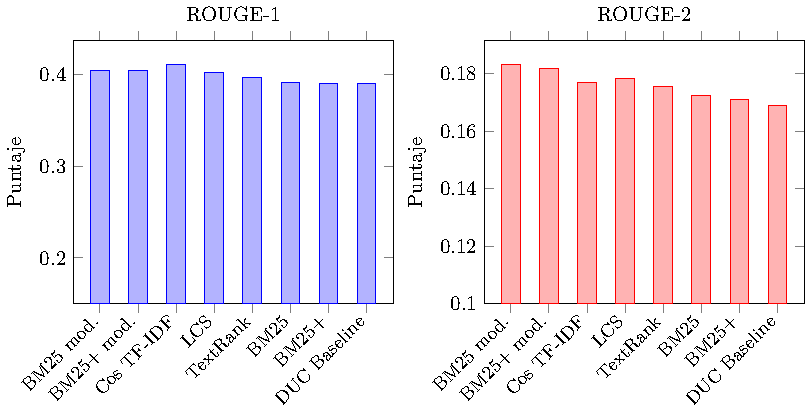
\includegraphics[width=1\textwidth]{rouge-scores.pdf}
    \caption{Comparación de métricas.}
\end{figure}



\section{Conclusiones}
En este trabajo se analizaron variantes al algoritmo de TextRank. A partir del mismo se propusieron e implementaron optimizaciones cuyos resultados fueron significativos: se obtuvo una mejoría del 2,92\% por sobre el método original. Este número es notable si se tiene en cuenta que TextRank por sí solo performa 2,84\% por sobre el estándar de comparación (baseline).

Las evaluaciones fueron hechas con las mismas técnicas y conjuntos de datos utilizados en competencias internacionales, validando así las mediciones.

En base a estos resultados proponemos la utilización de BM25 o BM25+ junto con TextRank como herramienta para la generación de resúmenes automáticos. Los ejemplos analizados y las métricas obtenidas demuestran resultados a los obtenidos por la versión original del algoritmo TextRank sin costo alguno extra de tiempo de procesamiento. 

Queda para próximos trabajos explorar alternativas para la extracción de palabras claves, y el ensayo de distintos métodos algebraicos, haciendo uso del modelo del espacio vectorial.


\bibliography{report}{}
\bibliographystyle{babunsrt}


\end{document}
